\documentclass[11pt, a4paper]{article}

\usepackage[utf8]{inputenc}
\usepackage[T1]{fontenc}
\usepackage{hyperref}
\usepackage{url}
\usepackage{booktabs}
\usepackage{amsfonts}
\usepackage{nicefrac}
\usepackage{microtype}
\usepackage{xcolor}
\usepackage{graphicx}
\usepackage{amsmath}
\usepackage{caption}
\usepackage{subcaption}
\usepackage{svg}
\usepackage[spanish, es-tabla]{babel}

\usepackage[margin=2.5cm]{geometry}

\hypersetup{
    colorlinks=true,
    linkcolor=blue,
    filecolor=magenta,      
    urlcolor=blue,
}

\begin{document}

\begin{titlepage}
    \centering
    \vspace*{2cm}
    
    {\scshape\Large Universidad Carlos III de Madrid \par}
    \vspace{0.5cm}
    {\scshape\large Departamento de Teoría de la Señal y Comunicaciones \par}
    \vspace{2cm}
    
    {\scshape\Large Aprendizaje Profundo para el Análisis de Imágenes  \par}
    \vspace{0.5cm}
    {\large Curso 2025/2026 \par}
    
    \vspace{3cm}
    \rule{\textwidth}{0.4pt}\vspace*{-\baselineskip}\vspace{3.2pt}
    \rule{\textwidth}{1.6pt}\\[\baselineskip]
    {\huge\bfseries PROYECTO 2:\\[0.5cm] Evaluación del Impacto de Desastres Naturales mediante Detección de Objetos \par}
    \vspace{0.2cm}
    \rule{\textwidth}{1.6pt}\vspace*{-\baselineskip}\vspace{3.2pt}
    \rule{\textwidth}{0.4pt}
    
    \vspace{3cm}
    
    {\Large\itshape Autores:\par}
    \vspace{0.5cm}
    {\Large  Lucrezia Cosmi \quad \texttt{100576666@alumnos.uc3m.es}\par}
    {\Large  Favier Alejandro Rojas Cuan \quad \texttt{100505199@alumnos.uc3m.es}\par}
    {\Large  Alejandro Gonzalez Chima \quad \texttt{100451454@alumnos.uc3m.es}\par}
    
    \vfill
\end{titlepage}

\newpage

\section{Introducción y Metodología}

En esta segunda fase del proyecto, el enfoque evolucionó de la clasificación de parches aislados ($64\times64$ píxeles) a la Detección de Objetos. Este cambio de paradigma permite a la red procesar áreas geográficas más amplias ($512\times512$ píxeles), incorporando el contexto geoespacial necesario para diferenciar la infraestructura del entorno (\textit{background}).

Para abordar este problema se implementó la arquitectura \textbf{Faster R-CNN}, un detector de dos etapas compuesto por una red extractora de características (\textit{Backbone}), una Red de Proposición de Regiones (RPN) y un módulo de \textit{RoI Pooling} para la clasificación y regresión final.

\section{Manejo de Dataset}

Dada la rigidez estructural que exige el \textit{framework} \texttt{torchvision} para la detección de objetos, se optó por un diseño de software basado en la separación de responsabilidades, dividiendo la carga de datos en dos clases:

\begin{itemize}
    \item \textbf{\texttt{xBDDataset} (Clase Base):} Encargada del procesamiento primario. Extrae las coordenadas de los polígonos originales y genera ventanas de $512\times512$ píxeles normalizadas.
    \item \textbf{\texttt{xBDDetectionDataset} (Clase Adaptadora):} Transforma las salidas genéricas al formato estricto requerido por Faster R-CNN. Específicamente:
    \begin{itemize}
        \item \textbf{Gestión del Background:} Desplaza las etiquetas originales (\texttt{labels + 1}), reservando estrictamente la clase \texttt{0} para el ``Fondo''. Esto permite a la red suprimir automáticamente las predicciones sobre carreteras o vegetación.
        \item \textbf{Filtrado Espacial:} Elimina \textit{bounding boxes} cuyo ancho o alto queda reducido a 0 píxeles tras el recorte de las ventanas, previniendo divisiones por cero (\texttt{NaN}) en la función de pérdida.
        \item \textbf{Estructura del \texttt{target} y \texttt{collate\_fn}:} Se empaquetaron las anotaciones en un diccionario estricto con las claves \texttt{"boxes"}, \texttt{"labels"} y \texttt{"area"}. Asimismo, se implementó una función \texttt{collate\_fn} a medida (\texttt{tuple(zip(*batch))}) para evitar la concatenación matricial de imágenes con un número variable de edificios.
    \end{itemize}
\end{itemize}

\section {Arquitectura}

\begin{figure}[hbt!]
    \centering
    % TODO: SUSTITUIR LA LÍNEA DE ABAJO POR TU IMAGEN
    % \rule{\linewidth}{6cm} % PLACEHOLDER PARA LA IMAGEN DEL DIAGRAMA
    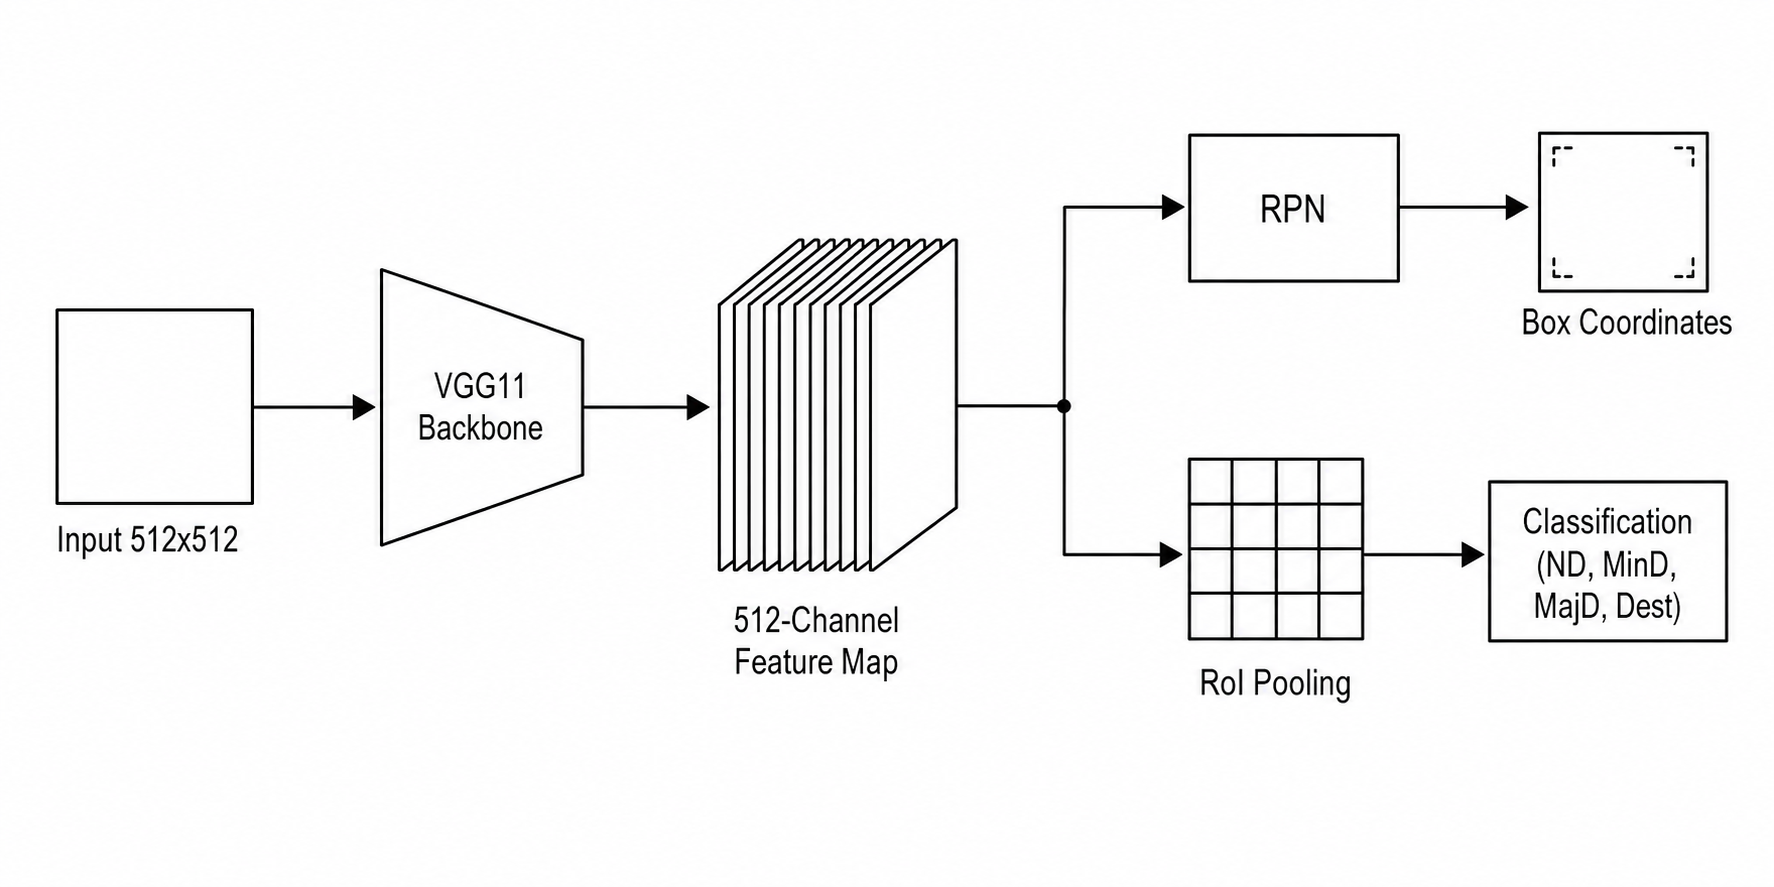
\includegraphics[width=\textwidth]{img/esquema.png}
    \caption{Esquema conceptual del flujo de datos. La imagen de entrada atraviesa el \textit{backbone} VGG11, generando un mapa de características de 512 canales. Este mapa alimenta de manera bifurcada a la RPN (para localización) y al \textit{RoI Pooling} (para clasificación final).}
    \label{fig:diagrama}
\end{figure}

\subsection{Reutilización del Backbone (VGG11)}
Para la extracción de características, se reutilizó la arquitectura \texttt{VGG11\_bn} sometida a \textit{fine-tuning} en el proyecto anterior, eliminando sus capas densas finales. De este modo, la imagen RGB se transforma en un tensor de características de \textbf{512 canales} de profundidad. 
\subsection{Adaptación del Generador de Anclas (\textit{Anchors})}
Los hiperparámetros por defecto de Faster R-CNN suelen estar optimizados para objetos de gran tamaño. Dado que la infraestructura vista desde arriba ocupa áreas reducidas, se definió un \texttt{AnchorGenerator} con escalas específicas \texttt{(16, 32, 64, 128, 256)} y relaciones de aspecto simétricas \texttt{(0.5, 1.0, 2.0)}. Teóricamente, esto fuerza a la RPN a generar \textit{priors} geométricos mejor adaptados a techos y naves industriales, reduciendo el esfuerzo matemático en la regresión de las coordenadas.

\section{Criterios de Evaluación}

Para validar las predicciones de forma robusta, no basta con evaluar la clase predicha. Se implementó una evaluación geométrica basada en la métrica \textbf{IoU (\textit{Intersection over Union})}. Se considera una predicción como ``Acierto'' (Verdadero Positivo) únicamente si cumple dos condiciones simultáneas:

\begin{enumerate}
    \item \textbf{Localización:} El área de solapamiento entre la caja predicha y la real es $\ge 50\%$ (\texttt{IoU >= 0.5}).
    \item \textbf{Clasificación:} La clase de daño predicha coincide exactamente con la etiqueta del \textit{Ground Truth}.
\end{enumerate}

\section{Análisis de Resultados y Limitaciones Observadas}

Durante las inferencias en el conjunto de test, el modelo evidenció comportamientos que subrayan la complejidad del problema:

\begin{itemize}
    \item \textbf{Capacidad de localización (RPN):} El modelo logró aislar las estructuras de manera razonable, discriminando con éxito los edificios del fondo gracias al ajuste de las anclas.
    \item \textbf{Sesgo hacia la clase mayoritaria:} En la fase de clasificación, el modelo mostró una fuerte tendencia a predecir la clase \textit{No-Damage} (clase mayoritaria, $\sim 83\%$). Al no introducir penalizaciones asimétricas en la pérdida de Faster R-CNN, el modelo minimiza su error global sesgándose hacia la clase dominante.
    \item \textbf{Problema de fragmentación:} Se observó que edificaciones de gran tamaño a menudo son fragmentadas en múltiples cajas pequeñas. Al carecer de una Red Piramidal de Características (FPN), el modelo tiende a identificar texturas locales (segmentos de tejado) en lugar de comprender la geometría global.
\end{itemize}

\begin{figure}[hbt!]
    \centering
    % TODO: SUSTITUIR LA LÍNEA DE ABAJO POR TU IMAGEN
    % \rule{\linewidth}{8cm} % PLACEHOLDER PARA LA COMPARATIVA PREDICCIÓN VS GT
    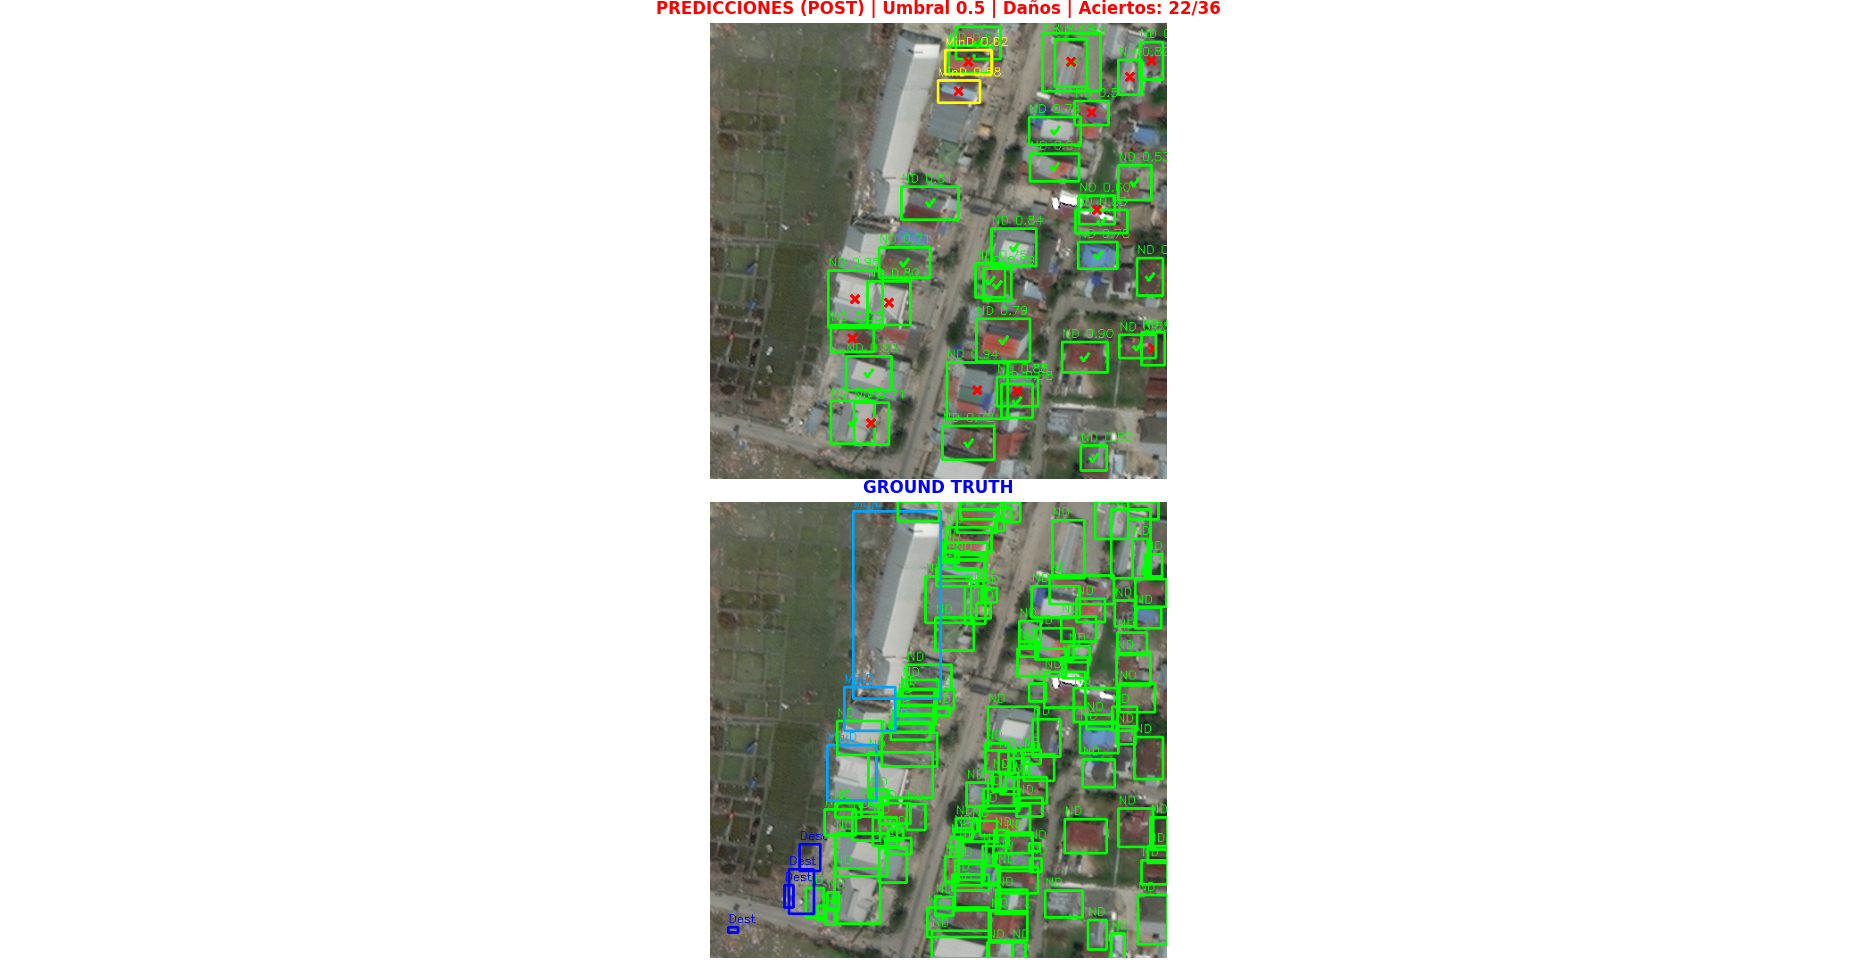
\includegraphics[width=0.9\textwidth]{img/figura_2.png}
    \caption{Comparativa de inferencia (arriba) frente a anotaciones \textit{Ground Truth} (abajo). Se aprecia una correcta localización espacial (\textit{bounding boxes} ajustados), pero una alta tasa de fallos en clasificación (cruces rojas) debido al sesgo generalizado del clasificador hacia la clase \textit{No-Damage}.}
    \label{fig:pred_vs_gt}
\end{figure}

\begin{figure}[hbt!]
    \centering
    % TODO: SUSTITUIR LA LÍNEA DE ABAJO POR TU IMAGEN
    % \rule{0.6\linewidth}{6cm} % PLACEHOLDER PARA IMAGEN FRAGMENTACIÓN
     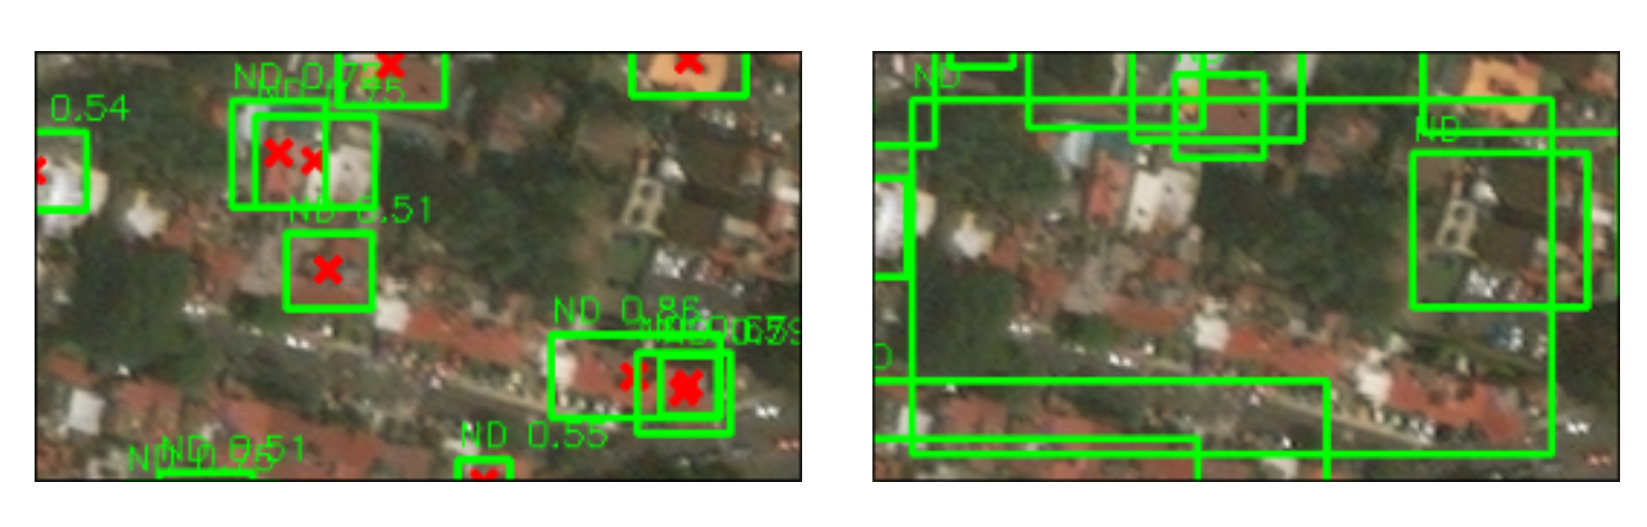
\includegraphics[width=0.6\textwidth]{img/figura_3.png}
    \caption{Fenómeno de fragmentación visual (predicciones a la izquierda, \textit{bounding boxes} reales a la derecha). Al carecer de un módulo FPN, la red clasifica la textura local del tejado generando múltiples detecciones sobre una misma infraestructura en lugar de un único \textit{bounding box} global.}
    \label{fig:fragmentacion}
\end{figure}

\section{Trabajo Futuro y Líneas de Mejora}

Dado que el dataset esta irremediablemente imbalanceado, la principal mejora para este proyecto que se propone es la implementación de FPN. Es necesario sustituir el \textit{backbone} actual por uno basado en \texttt{ResNet50} con \textit{Feature Pyramid Network} (FPN), fusionando la resolución espacial de las capas tempranas con la semántica de las profundas para otorgar invarianza de escala y reducir el efecto de fragmentación.

\end{document}
